\documentclass{beamer}
\usepackage[utf8]{inputenc}
\usetheme{Boadilla}
\usecolortheme{seahorse}
\usepackage[french]{babel}
%\usepackage{kpfonts}
\usepackage{tikz}

\usepackage{amsmath} % load the AMS math package
\usefonttheme{professionalfonts} % use the same font for math as in regular LaTeX document
\usepackage{unicode-math} % load a Unicode math font package
%\setmathfont{Latin Modern Math}



\title[Les technologies dans les vignobles (FLE)]{Les technologies dans les vignobles}
\author[Isai Gordeev]{Isai Gordeev\\X22}
\institute[]{École Polytechnique\\ Palaiseau}
\date{\today}

\begin{document}
	
	\begin{frame}
		\titlepage
	\end{frame}
	
	\begin{frame}
		\frametitle{Plan}
			\tableofcontents
	
	\end{frame}


	\section{But?}
	
	
	\begin{frame}
		\frametitle{But?}
		\begin{center}
Pourquoi utiliser la technologie si les ancêtres fabriquaient du vin en leur absence et surtout écrivaient des poèmes en honorant le vin charmant?
		\end{center}
	
		\begin{figure}
		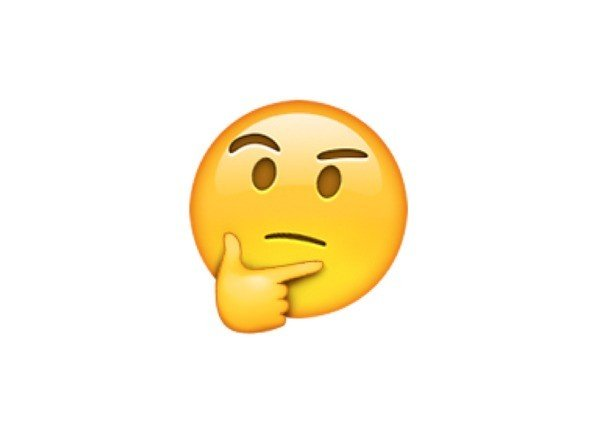
\includegraphics[width=0.8\textwidth]{1}
		\label{fig:example}
		\end{figure}
		
	\end{frame}


	\begin{frame}
	\frametitle{But?}
	\begin{center}
		Parce que on veut contrôler tout (y compris la quantité et la qualité du vin)
	\end{center}
	
	\begin{figure}
		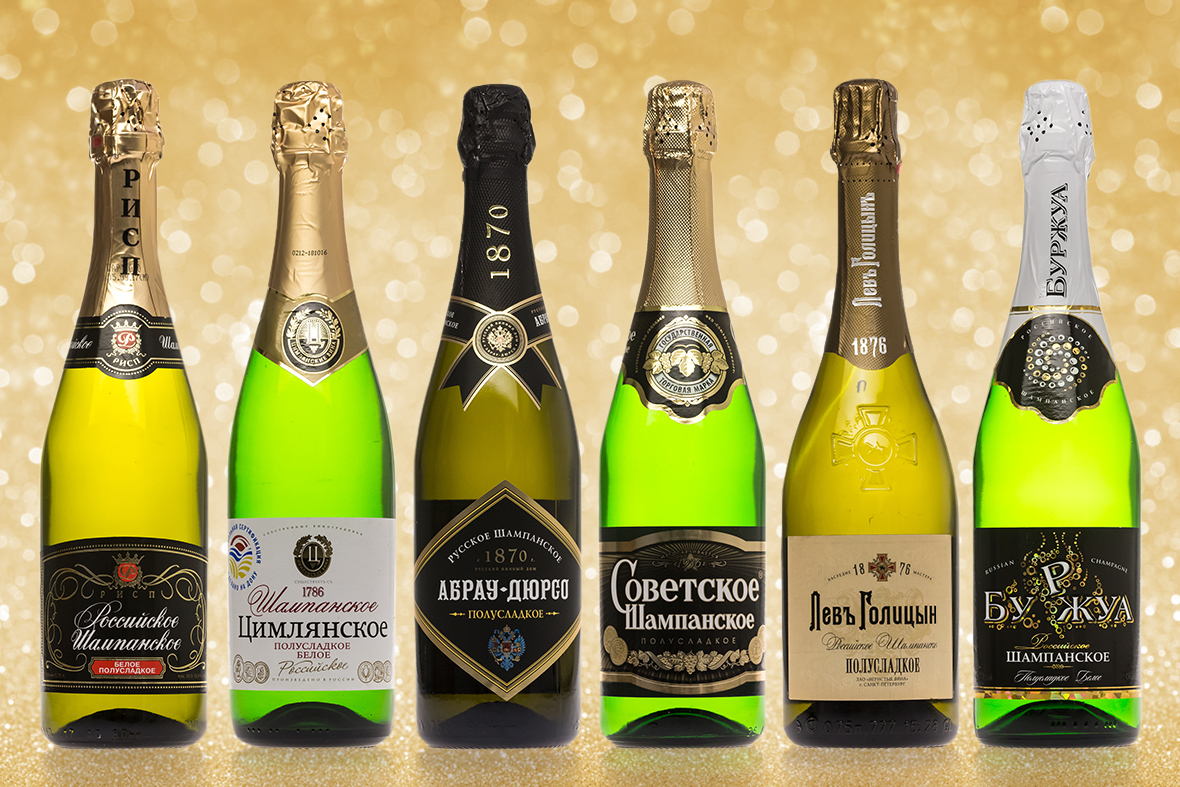
\includegraphics[width=0.7\textwidth]{cringevin}
		\label{fig:example}
	\end{figure}
	
\end{frame}


	\section{La Petite Histoire du Vin}

	\begin{frame}
	\frametitle{La Petite Histoire du Vin}
	\begin{itemize}
		\item Antiquité: Les techniques rudimentaires, mais elles sont les bases de l'industrie vinicole.
		\item 17e siècle: L'utilisation de bouteilles en verre pour conserver le vin. 
		\item 19e siècle: Les avancées importantes dans la distribution du vin.
		\item Années 1980 : L'adoption de la technologie informatique dans la gestion des vignobles et des caves
		\item Années 2000 : L'utilisation de capteurs, de drones et de technologies de surveillance avancées.
		\item Années 2010 : L'intelligence artificielle et l'analyse de données
	\end{itemize}
	
	\end{frame}


	\begin{frame}
	\frametitle{La Petite Histoire du Vin}
	\begin{itemize}
		\item \alert<1>{Antiquité: Les techniques rudimentaires, mais elles sont les bases de l'industrie vinicole.}
		\item \alert<2>{17e siècle: L'utilisation de bouteilles en verre pour conserver le vin. }
		\item \alert<3> {19e siècle: Les avancées importantes dans la distribution du vin.}
		\item  \alert<4>{Années 1980 : L'adoption de la technologie informatique dans la gestion des vignobles et des caves}
		\item  \alert<5>{Années 2000 : L'utilisation de capteurs, de drones et de technologies de surveillance avancées.}
		\item \alert<6>{Années 2010 : L'intelligence artificielle et l'analyse de données}

	\end{itemize}
	
\end{frame}



	\section{Les technologies des années 2000 et plus loin..}
	
	\begin{frame}
	\frametitle{Les technologies des années 2000 et plus loin..}
	\begin{itemize}
		\item Capteurs et surveillance
		\item GPS et cartographie
		\item Drones
		\item Analyse de données et intelligence artificielle
	\end{itemize}
	
	\begin{figure}
		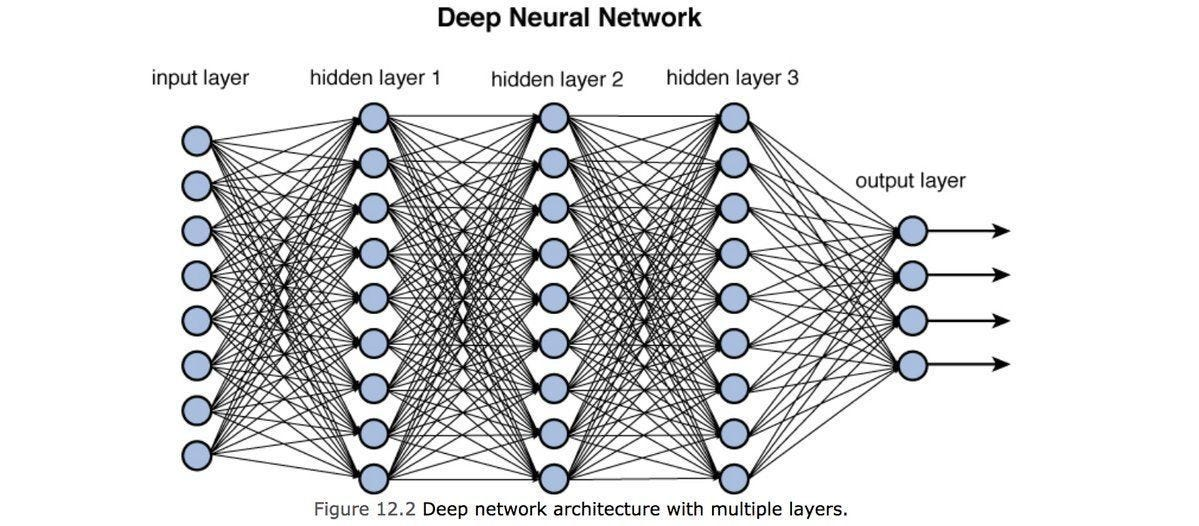
\includegraphics[width=0.8\textwidth]{neuron}
		\label{fig:example}
	\end{figure}
	
\end{frame}


	\begin{frame}
	\frametitle{Les technologies des années 2000 et plus loin..}
	\begin{itemize}
		\item \alert{Capteurs et surveillance}
		\item GPS et cartographie
		\item Drones
		\item Analyse de données et intelligence artificielle
	\end{itemize}
	
	\begin{figure}
		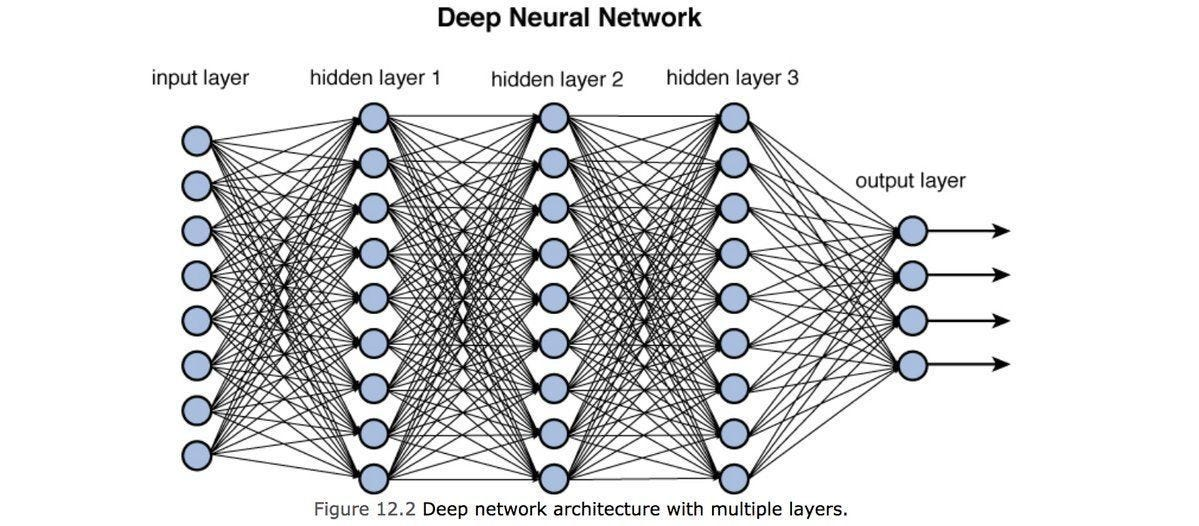
\includegraphics[width=0.8\textwidth]{neuron}
		\label{fig:example}
	\end{figure}
	
\end{frame}

	\subsection{Capteurs}


	\begin{frame}
	\frametitle{Capteurs}
	\begin{itemize}
		\item Capteurs de météo
		\item Capteurs de sol
		\item Capteurs de feuillage
		\item Capteurs de maturité des raisins
	\end{itemize}


		\begin{columns}[c]
	\column{.3\textwidth}
	\centering
	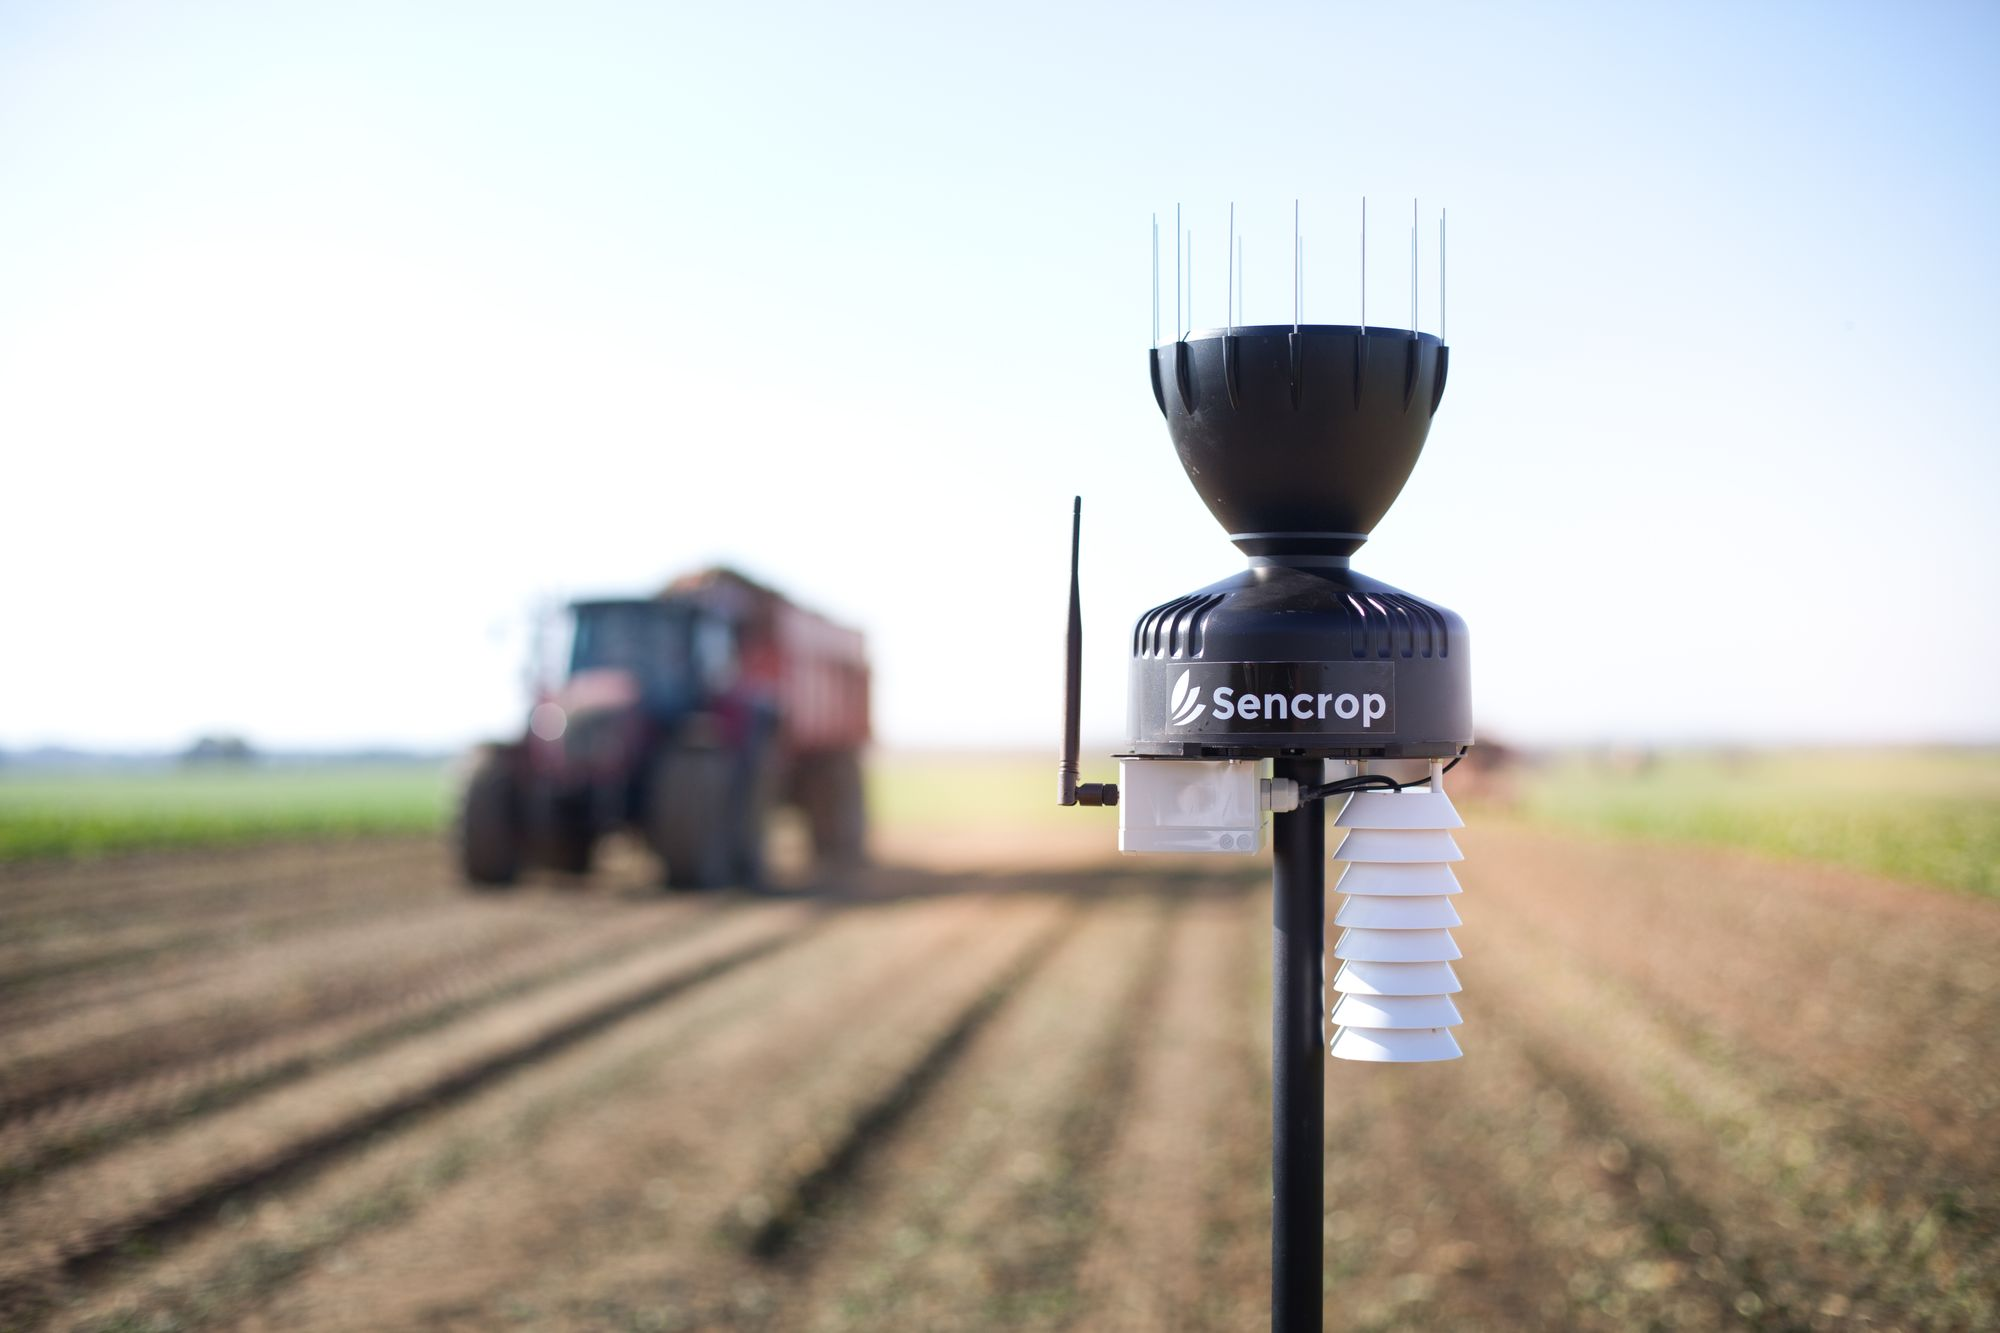
\includegraphics[width=\textwidth]{meteo}
	\column{.3\textwidth}
	\centering
	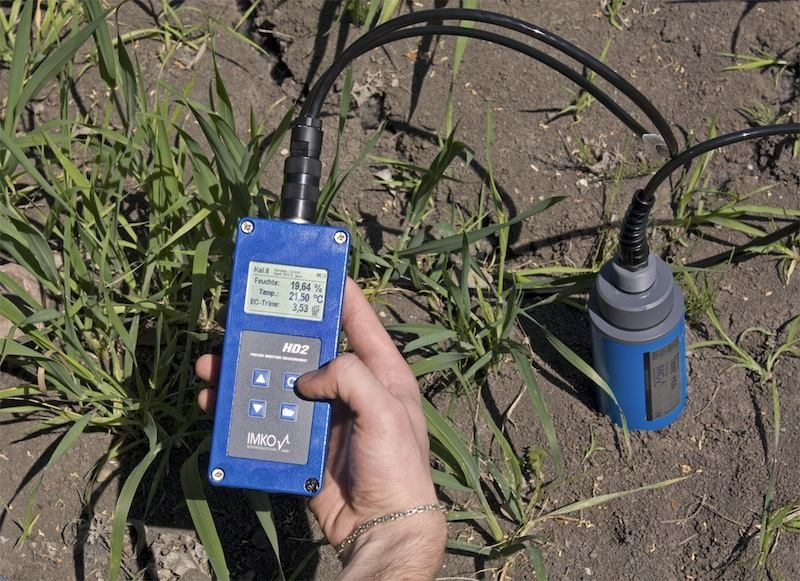
\includegraphics[width=\textwidth]{sol}
	\column{.3\textwidth}
	\centering
	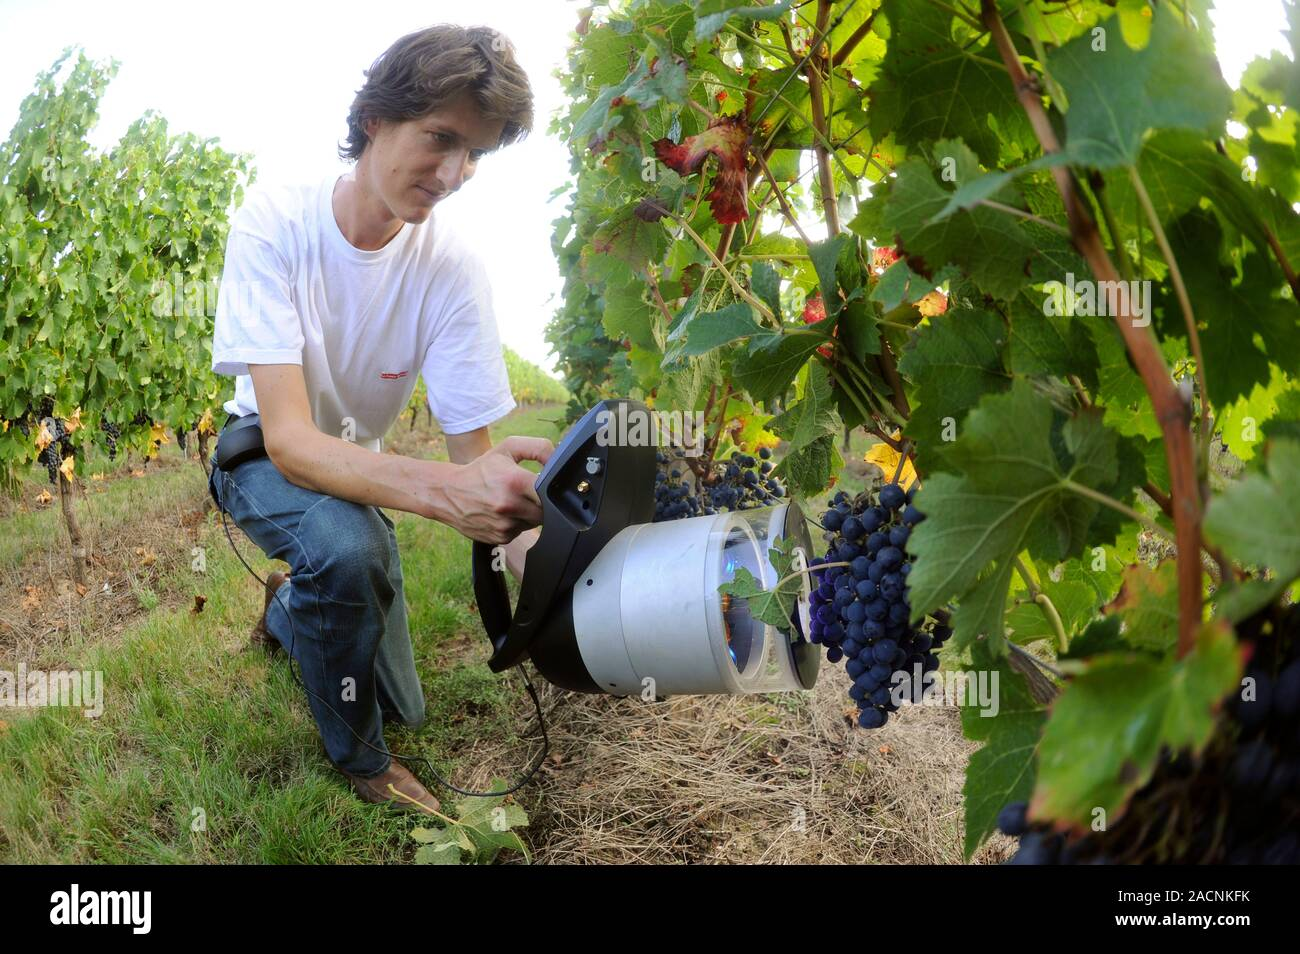
\includegraphics[width=\textwidth]{maturite}
	\end{columns}
	
	\end{frame}

		\subsection{GPS et cartographie}
		
		
			\begin{frame}
			\frametitle{Les technologies des années 2000 et plus loin..}
			\begin{itemize}
				\item Capteurs et surveillance
				\item \alert{GPS et cartographie}
				\item Drones
				\item Analyse de données et intelligence artificielle
			\end{itemize}
			
			\begin{figure}
				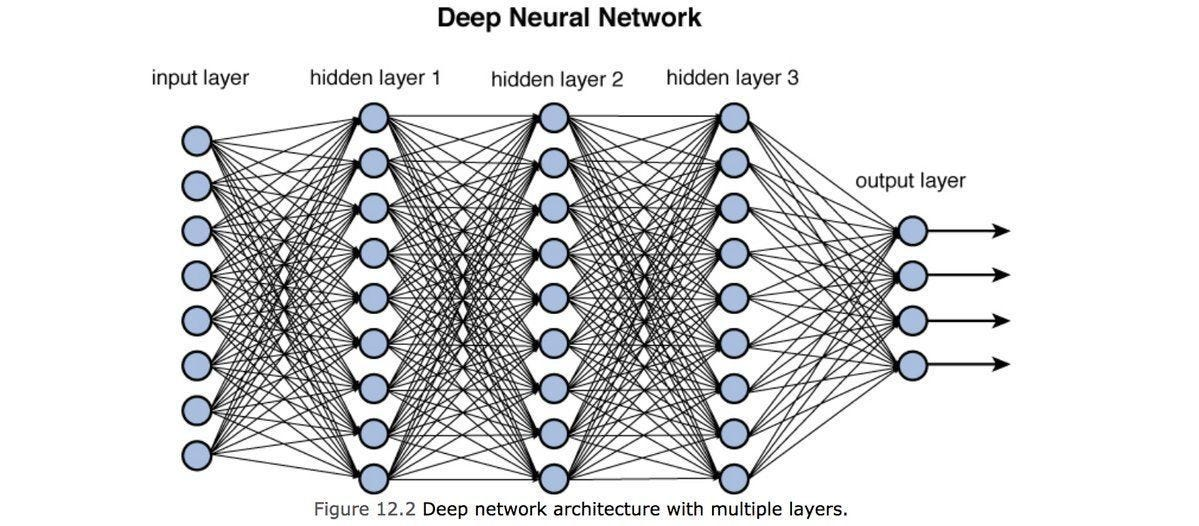
\includegraphics[width=0.8\textwidth]{neuron}
				\label{fig:example}
			\end{figure}
			
		\end{frame}
	
	
	\begin{frame}
		\frametitle{GPS et cartographie}
		\begin{itemize}
				\item Cartographie des parcelles de vignes
				\item Optimisation de l'irrigation
		\end{itemize}

	\begin{columns}[c]
		\column{.7\textwidth}
		\centering
		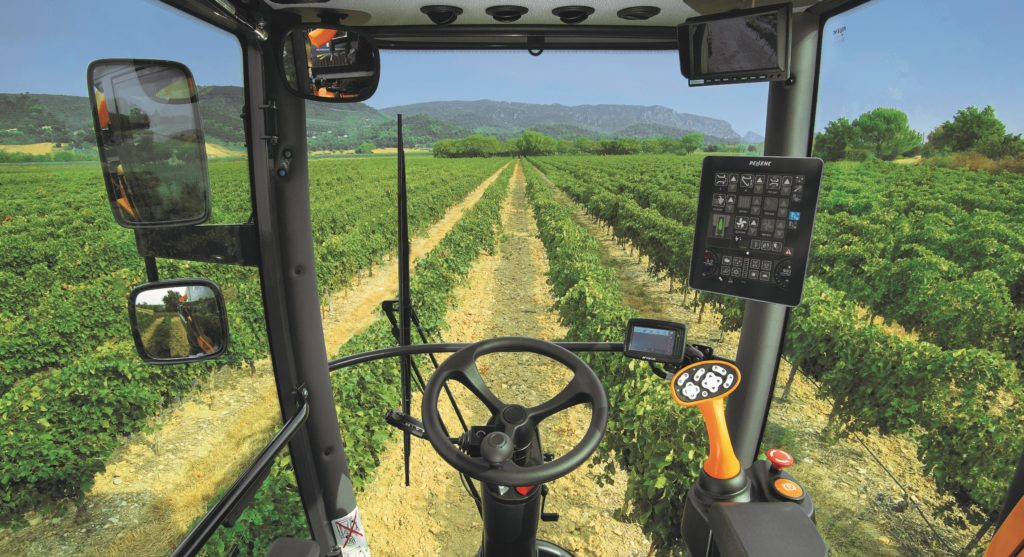
\includegraphics[width=\textwidth]{gps}
		\column{.2\textwidth}
		\centering
		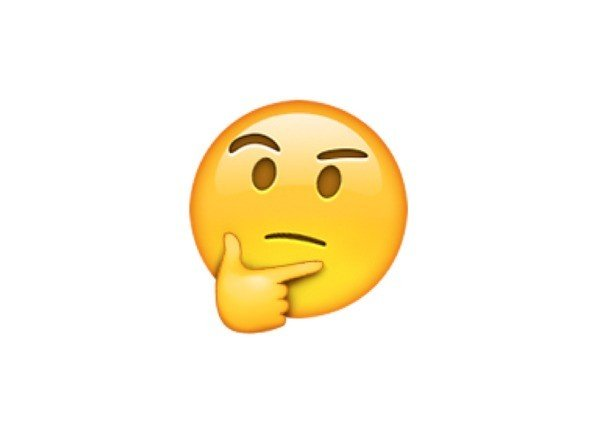
\includegraphics[width=\textwidth]{1}
	\end{columns}
	\end{frame}


			\begin{frame}
	\frametitle{Les technologies des années 2000 et plus loin..}
	\begin{itemize}
		\item Capteurs et surveillance
		\item GPS et cartographie
		\item \alert{Drones}
		\item Analyse de données et intelligence artificielle
	\end{itemize}
	
	\begin{figure}
	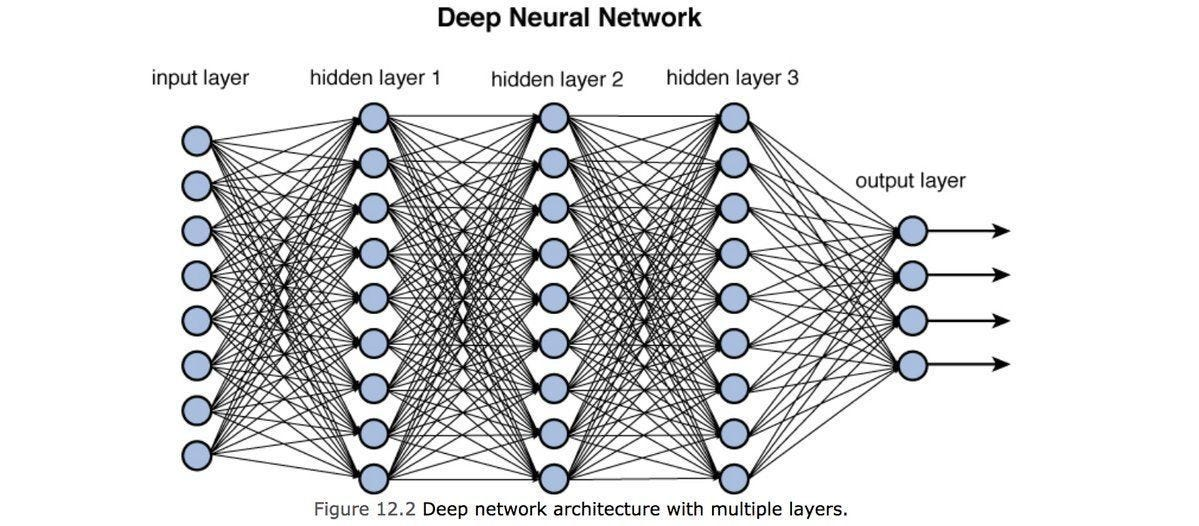
\includegraphics[width=0.8\textwidth]{neuron}
	\label{fig:example}
\end{figure}
	
\end{frame}

			\subsection{Drones}


		\begin{frame}
		\frametitle{Drones}
		\begin{itemize}
			\item Surveillance de la santé des vignes
			\item Gestion de l'irrigation
			\item Gestion de l'enherbement
		\end{itemize}
		
			\begin{figure}
			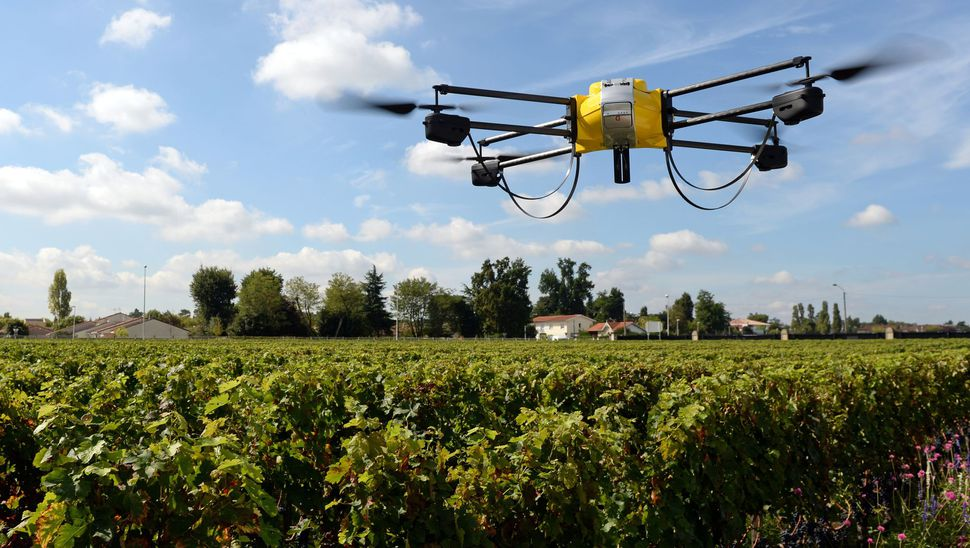
\includegraphics[width=0.8\textwidth]{drone}
			\label{fig:example}
		\end{figure}
		
	\end{frame}


			\begin{frame}
	\frametitle{Les technologies des années 2000 et plus loin..}
	\begin{itemize}
		\item Capteurs et surveillance
		\item GPS et cartographie
		\item Drones
		\item \alert{Analyse de données et intelligence artificielle}
	\end{itemize}
	
	\begin{figure}
		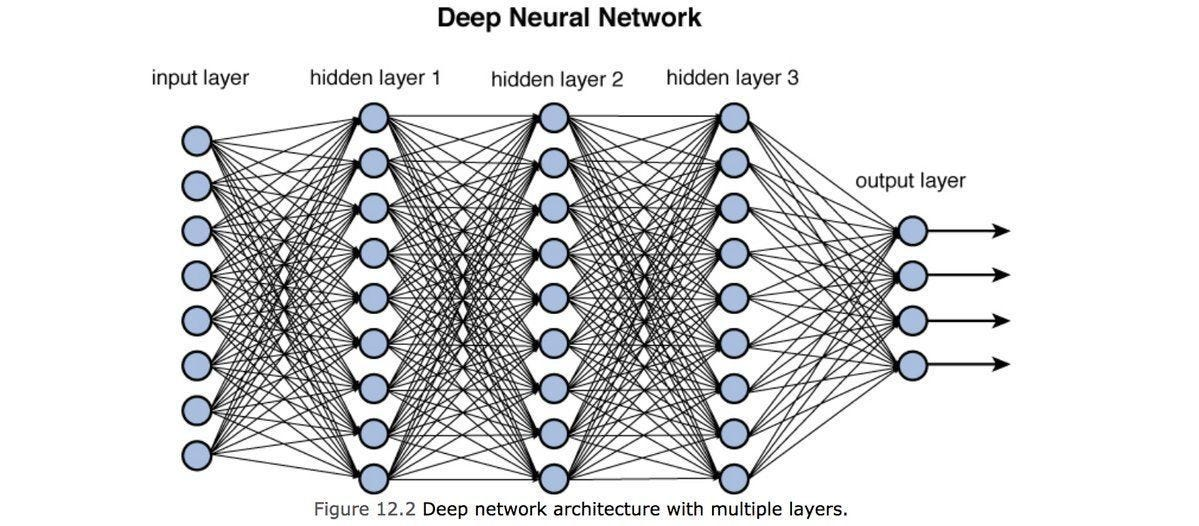
\includegraphics[width=0.8\textwidth]{neuron}
		\label{fig:example}
	\end{figure}
	
\end{frame}

		
		\subsection{Analyse de données et intelligence artificielle}

\begin{frame}
		\frametitle{Analyse de données et intelligence artificielle}
		\begin{itemize}
			\item Prévision des rendements
			\item Gestion de la cave
			\item Sélection des cépages
			\item ...
		\end{itemize}
	
	\begin{columns}[c]
	\column{.7\textwidth}
	\centering
	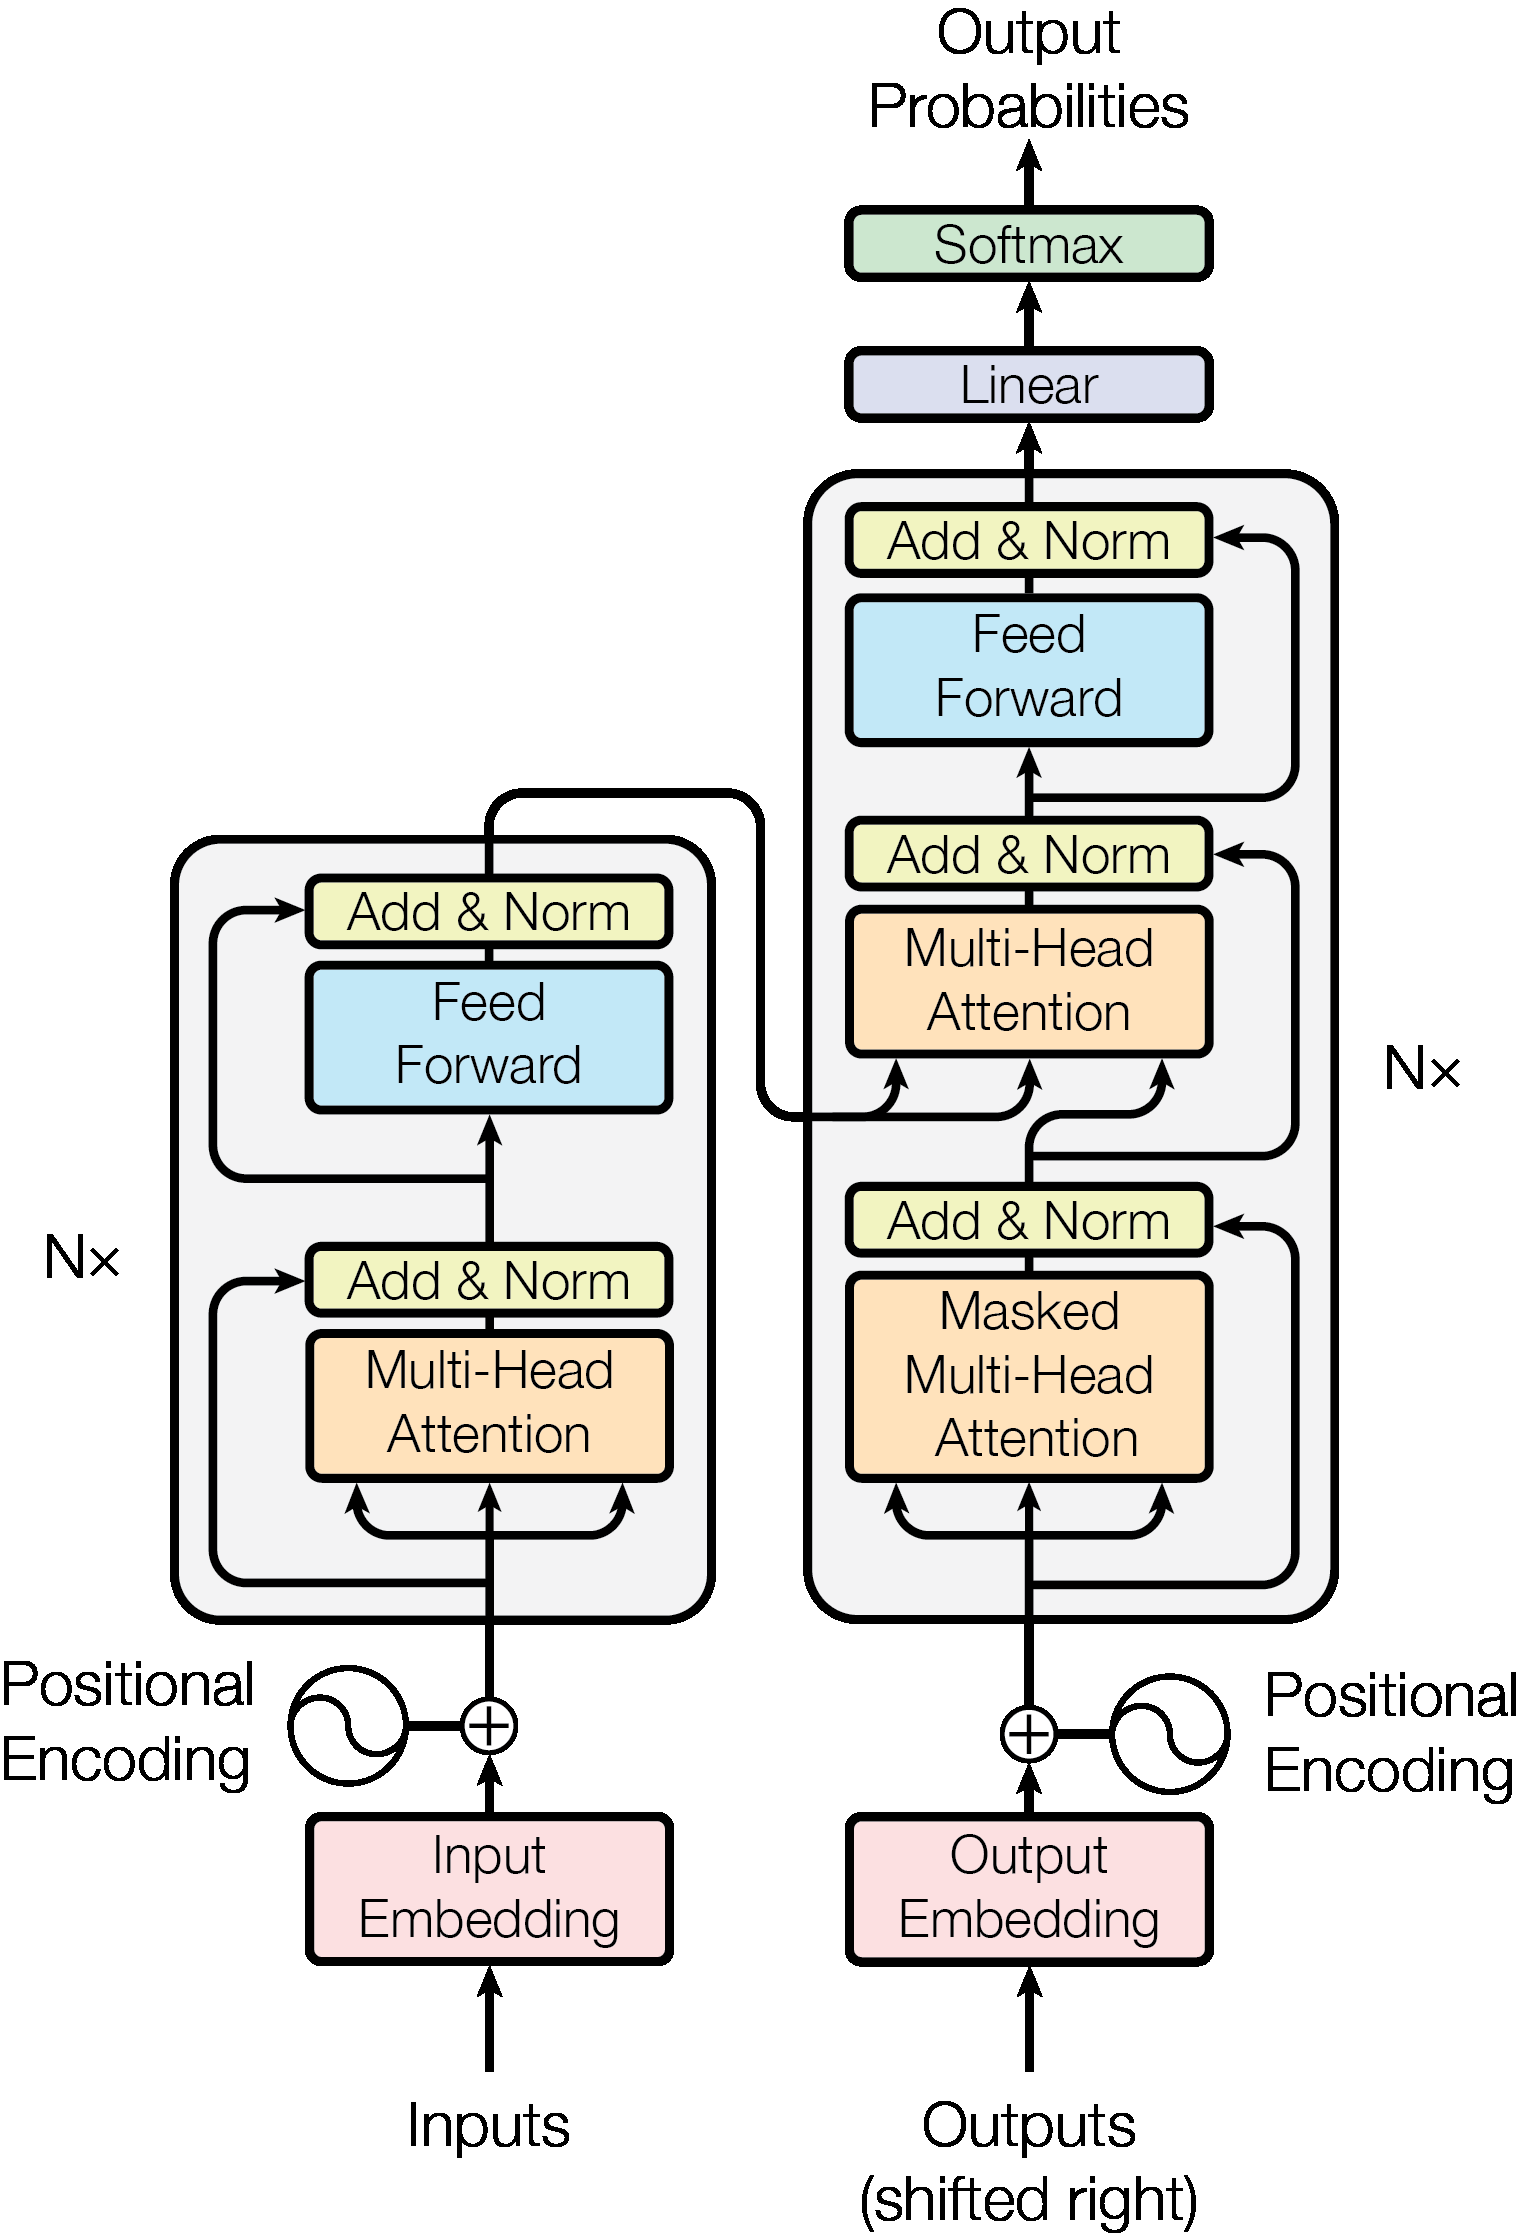
\includegraphics[width=\textwidth]{transformer}
	\column{.2\textwidth}
	\centering
	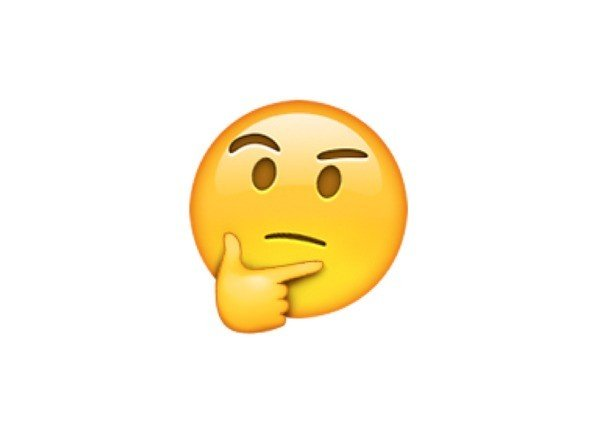
\includegraphics[width=\textwidth]{1}
\end{columns}
		
	\end{frame}


\begin{frame}
	\frametitle{Analyse de données et intelligence artificielle}
	\begin{itemize}
		\item ...
		\item Analyse sensorielle
		\item Optimisation des opérations viticoles
		\item Peut-être tout?
	\end{itemize}
	
	\begin{columns}[c]
		\column{.7\textwidth}
		\centering
		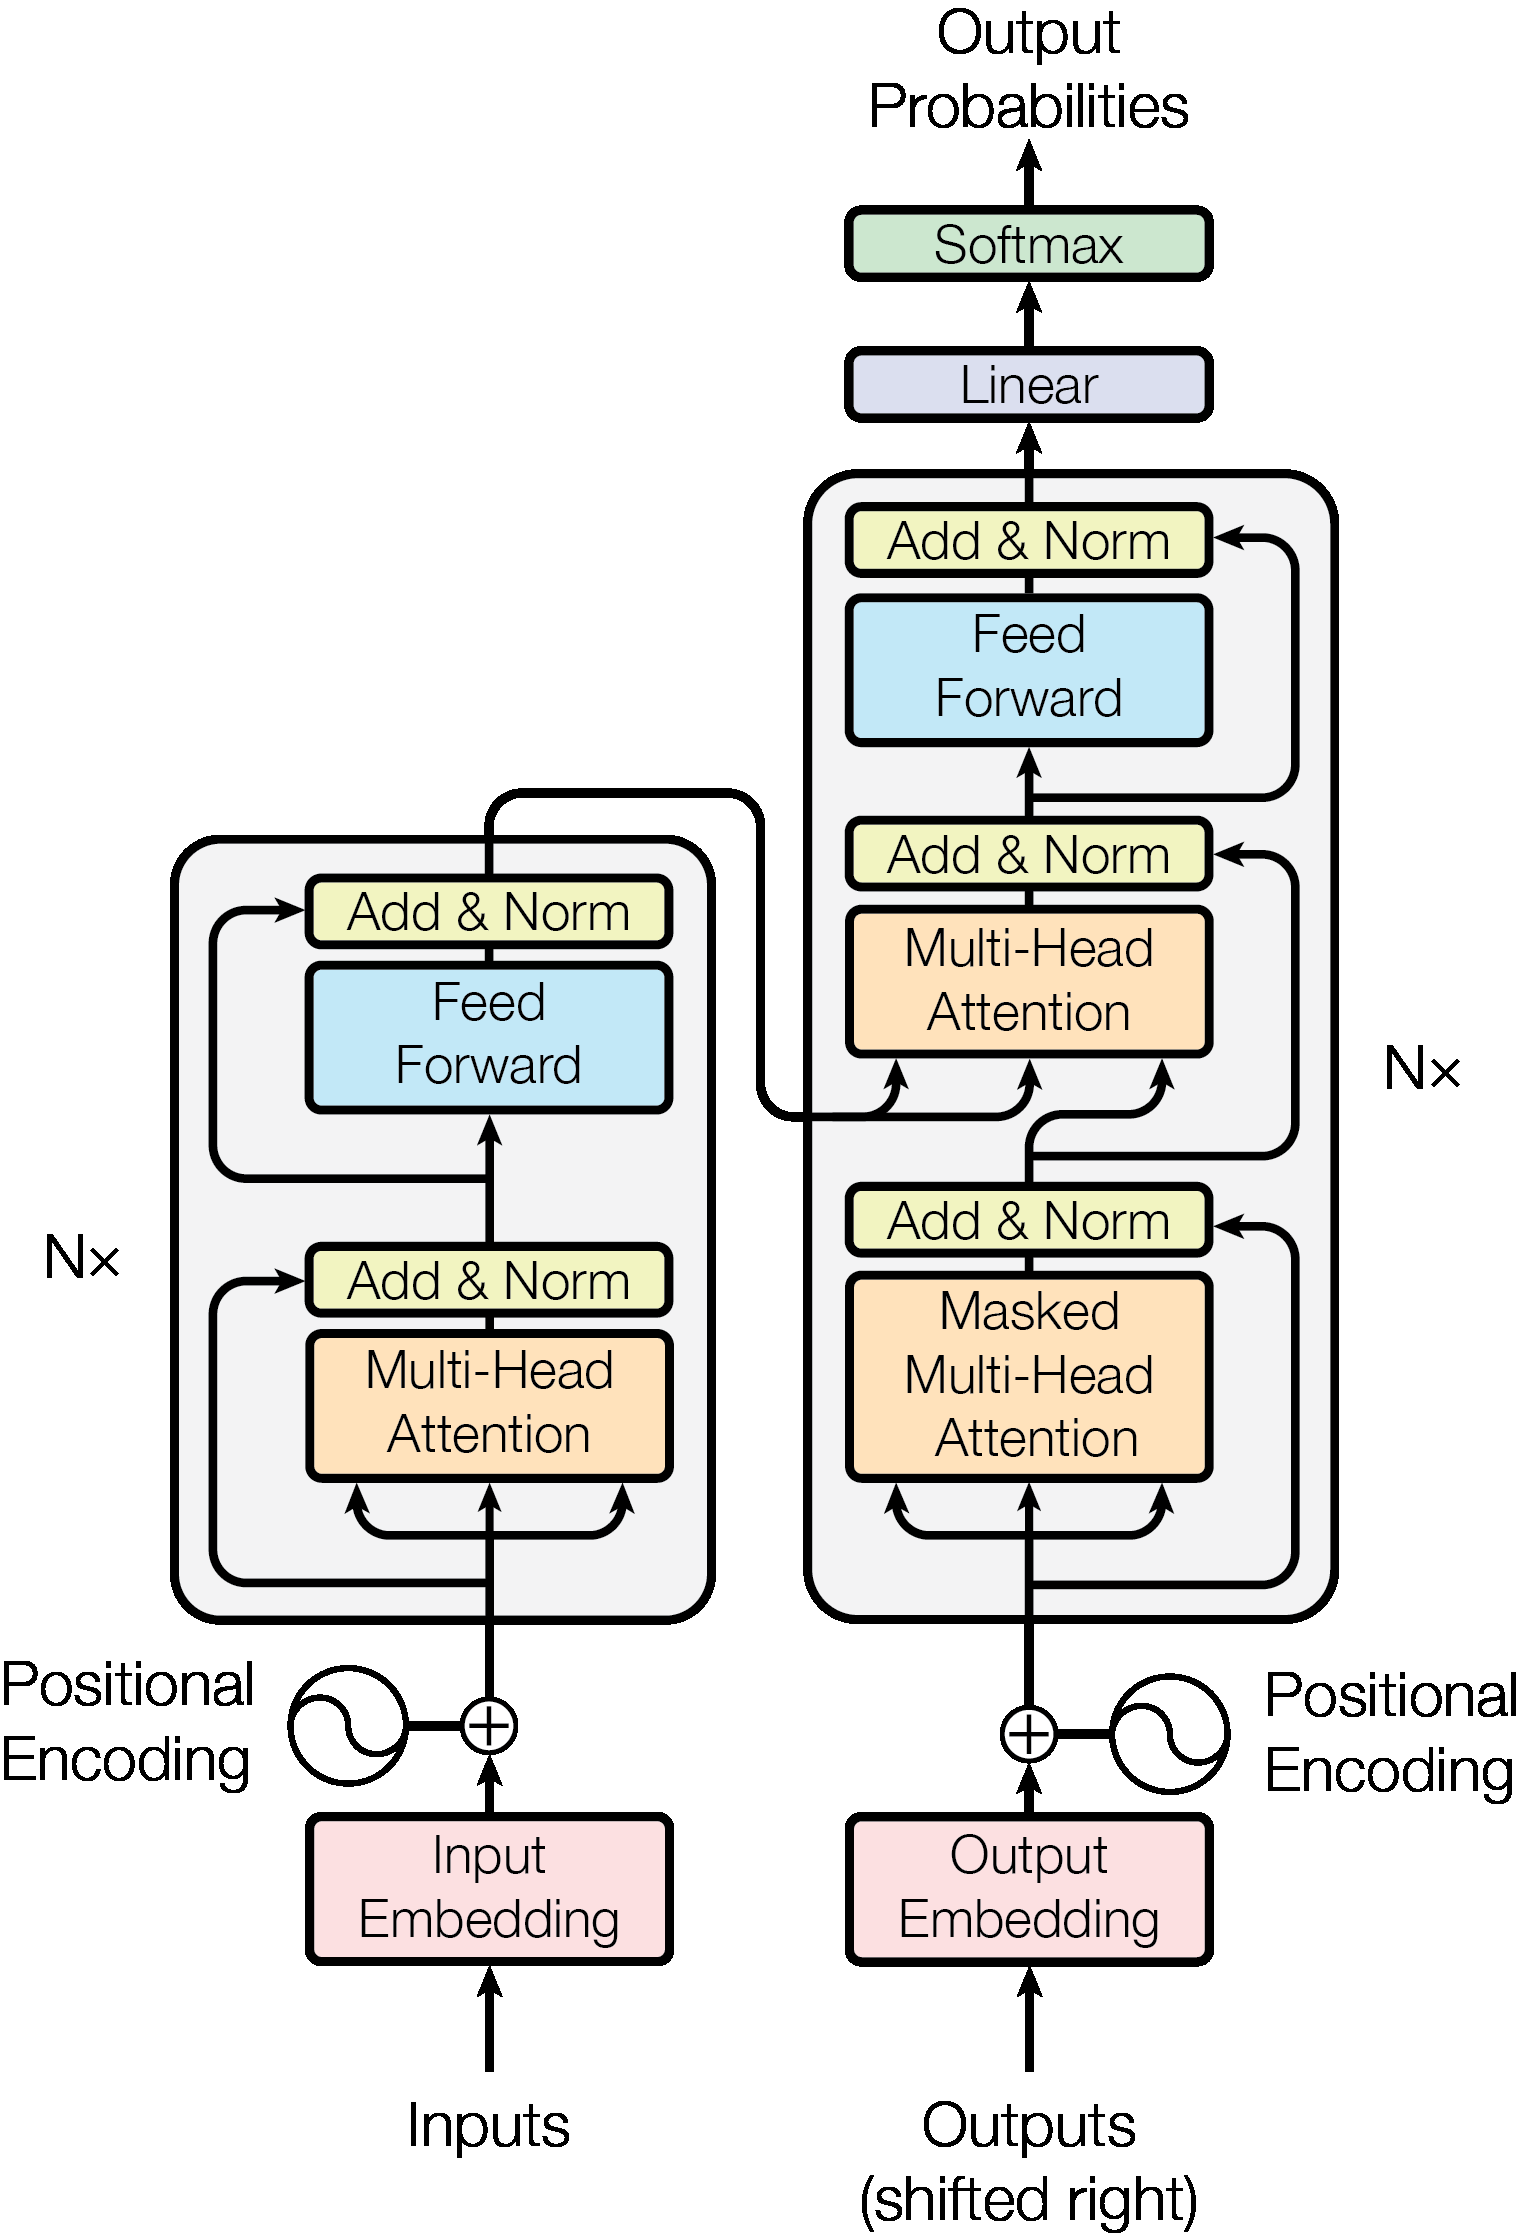
\includegraphics[width=\textwidth]{transformer}
		\column{.2\textwidth}
		\centering
		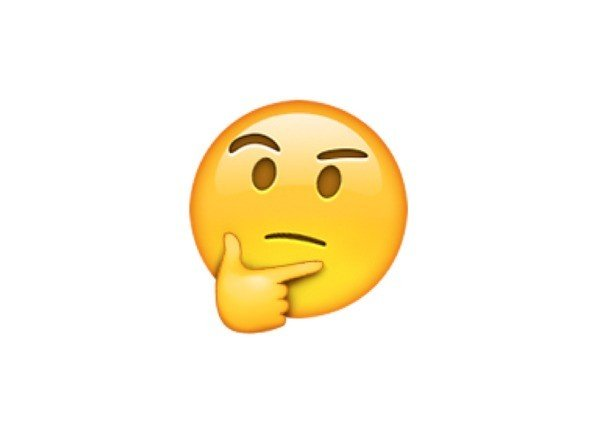
\includegraphics[width=\textwidth]{1}
	\end{columns}
	
\end{frame}

\section{DR-IACNN}

\begin{frame}
	\frametitle{Détecteur de maladies des feuilles de vigne}
	\begin{itemize}
		\item Premier modèle qui détaille les maladies 
		\item Basé sur ResNet 
		\item 80\% de précision
	\end{itemize}
	
			\begin{figure}
	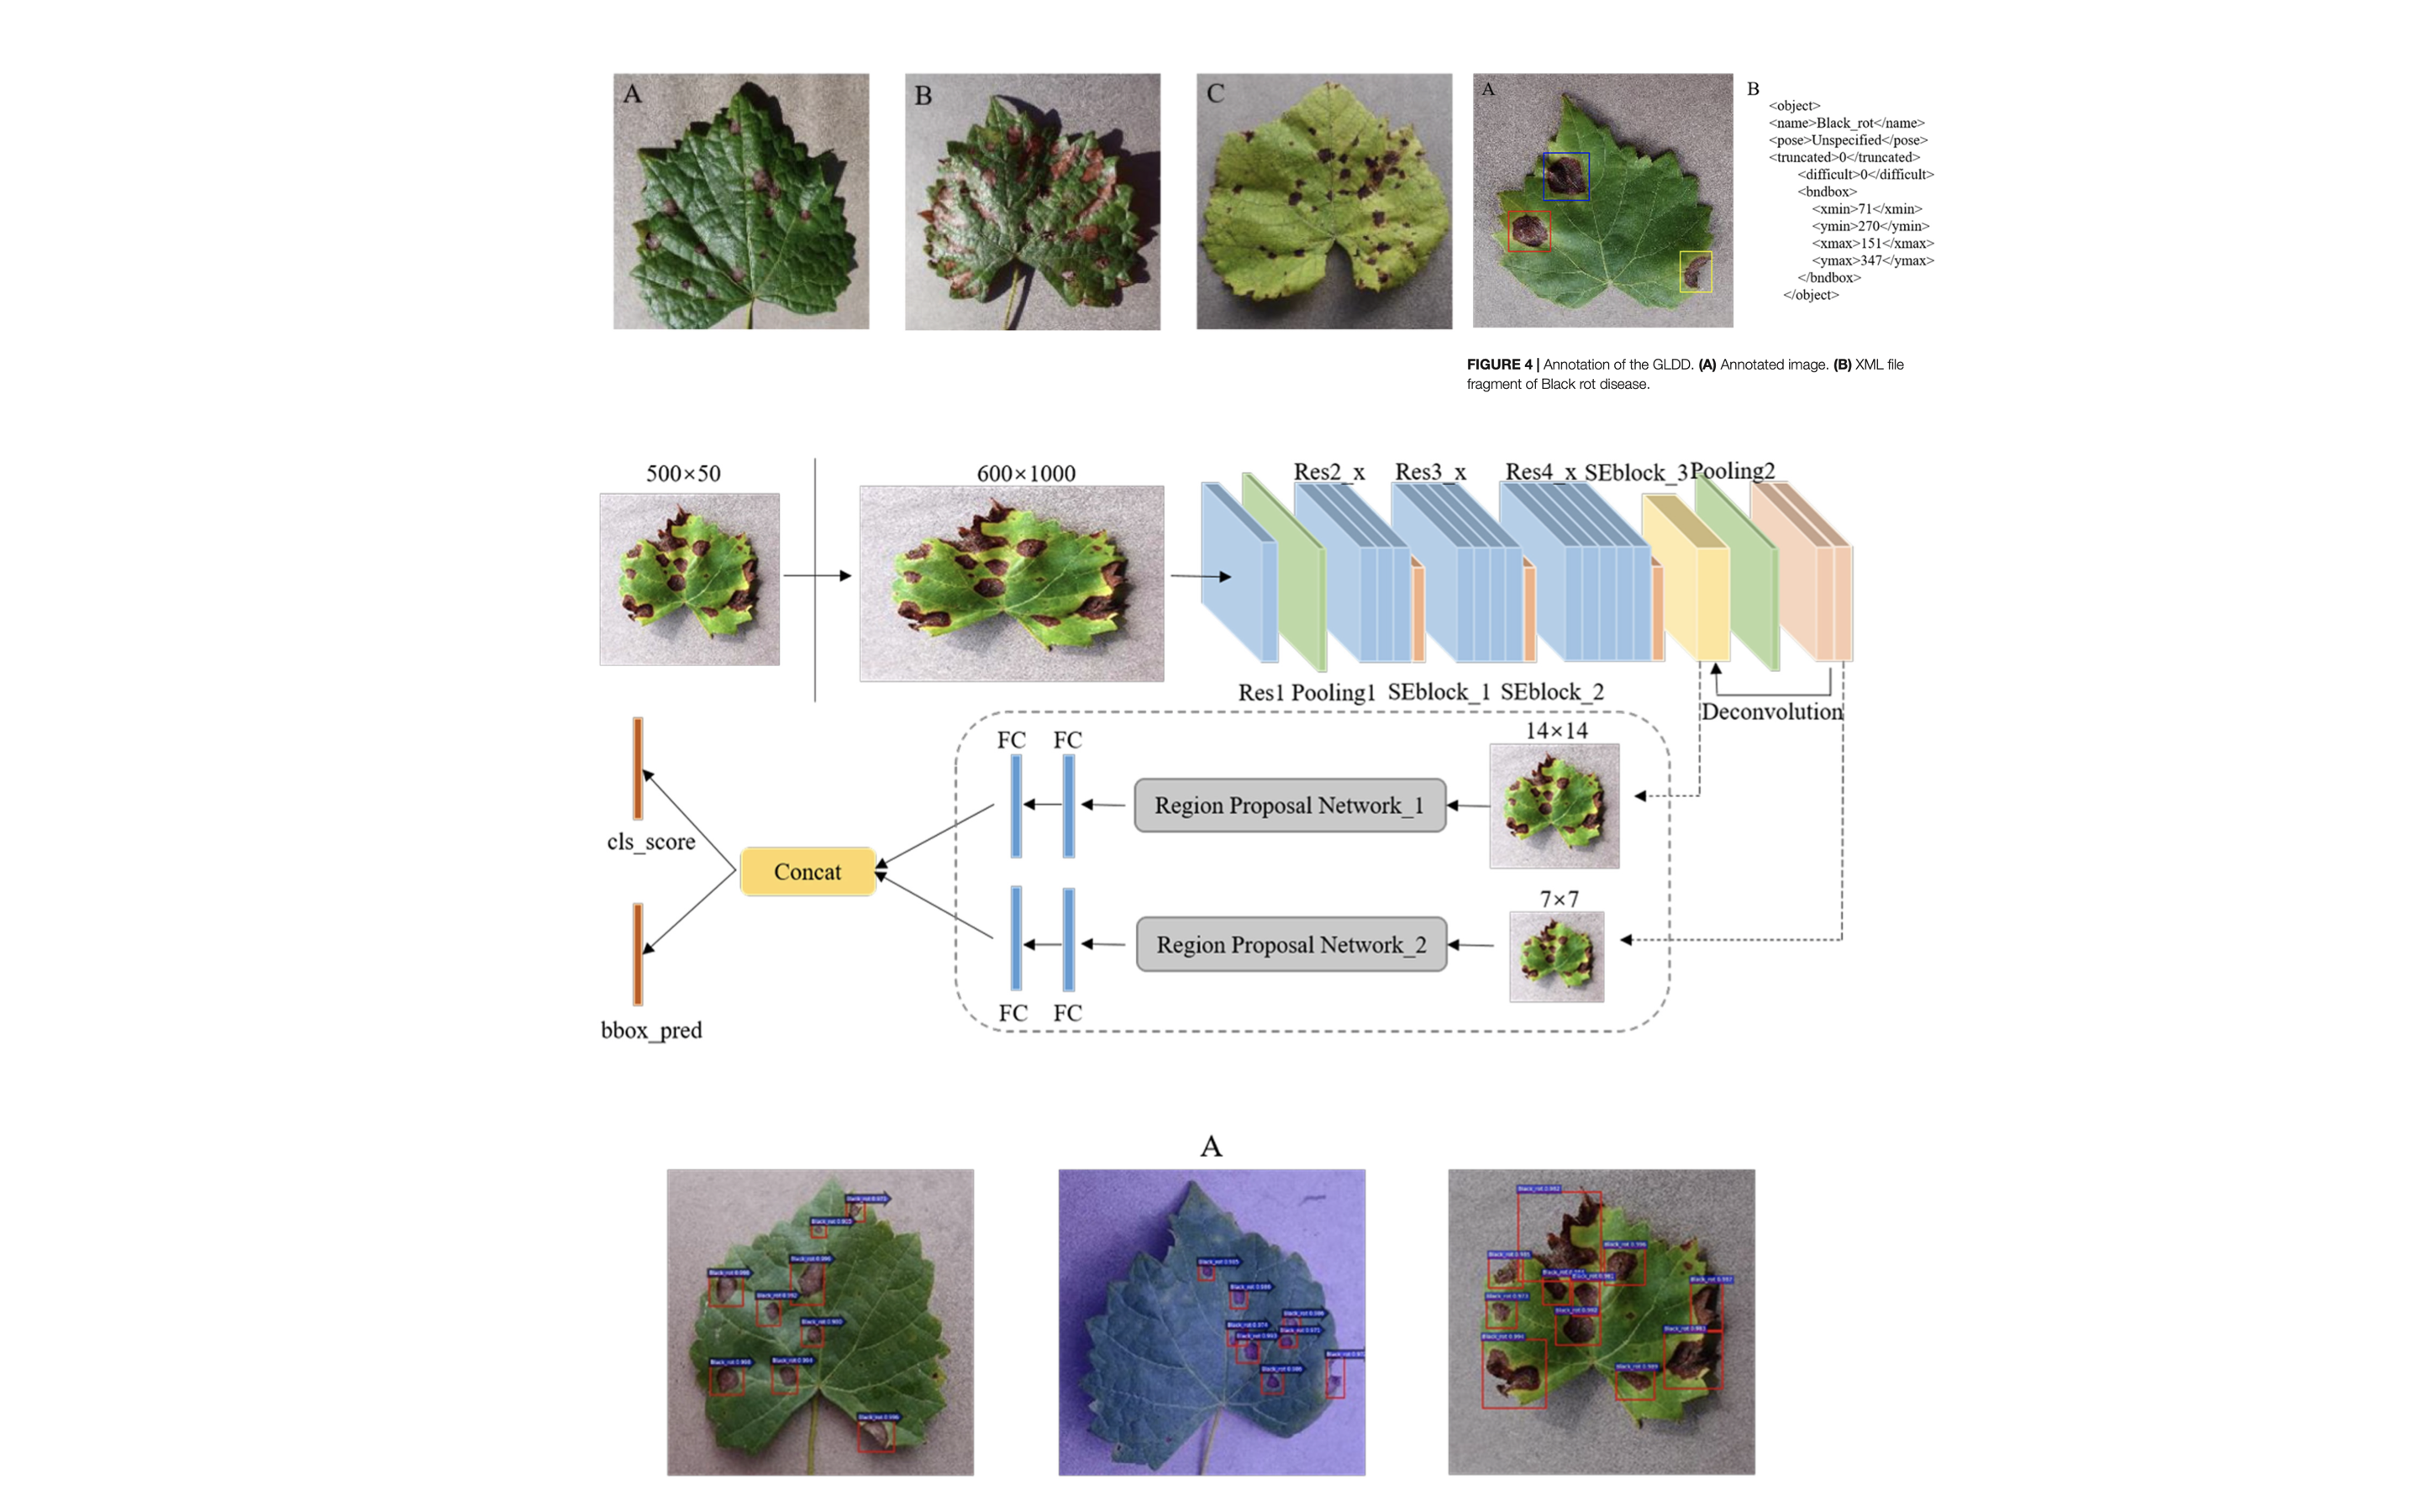
\includegraphics[width=0.8\textwidth]{reseau}
	\label{fig:example}
\end{figure}
	
\end{frame}


\section{Et le futur?}

		\begin{frame}
		\frametitle{Et le futur?}
		\begin{itemize}
			\item Agriculture durable
			\item Cépages résilients
			\item Recherche et développement
		\end{itemize}
	
		
			\begin{figure}
			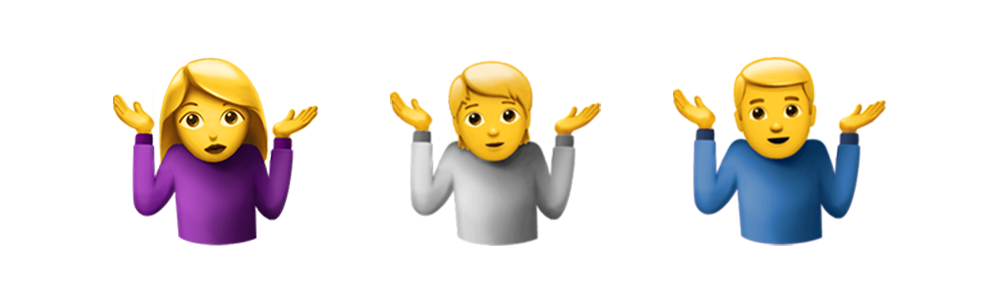
\includegraphics[width=0.8\textwidth]{futur}
			\label{fig:example}
		\end{figure}
	
	
	\end{frame}

	

	\begin{frame}
	\begin{center}
{\LARGE Merci pour votre attention }
	\end{center}
\end{frame}



	
\end{document}
